\documentclass[11pt,a4paper]{article}

\usepackage[margin=2.1cm]{geometry}
\usepackage[T1]{fontenc}
\usepackage[utf8]{inputenc}
\usepackage{lmodern}
\usepackage{microtype}
\usepackage{amsmath,amssymb,mathtools}
\usepackage{booktabs,array,tabularx}
\usepackage{xcolor}
\usepackage{tcolorbox}
\tcbuselibrary{skins,breakable}
\usepackage{tikz}
\usetikzlibrary{arrows.meta,positioning,calc}
\usepackage{fancyhdr}
\usepackage{hyperref}
\usepackage{enumitem}

% Academic color palette
\definecolor{navy}{HTML}{1B365D}
\definecolor{slate}{HTML}{2C5282}
\definecolor{tint}{HTML}{F4F7FA}
\definecolor{amber}{HTML}{8A5A00}
\definecolor{ambertint}{HTML}{FFFBEB}
\definecolor{greenink}{HTML}{1E5631}
\definecolor{greentint}{HTML}{F1F8F4}
\definecolor{crimson}{HTML}{9B1C1C}

\hypersetup{
  colorlinks=true,
  linkcolor=slate,
  urlcolor=slate,
  pdftitle={Class Notes: Physics-Informed Discovery of Ice Accretion and Shedding in Turbomachinery},
  pdfauthor={eqform Lecture Notes}
}

\pagestyle{fancy}
\fancyhf{}
\fancyhead[L]{\small\color{slate}\textsc{Class Notes: Ice Accretion \& Shedding Discovery (\texttt{eqform})}}
\fancyhead[R]{\small\color{slate}Turbomachinery \& Heat-Exchanger Multi-Physics}
\fancyfoot[C]{\small\thepage}
\renewcommand{\headrulewidth}{0.4pt}

\newtcolorbox{setupbox}[1]{
  breakable, enhanced, colback=tint, colframe=navy, boxrule=0.8pt, arc=3pt,
  left=8pt, right=8pt, top=6pt, bottom=6pt, fonttitle=\bfseries\color{white}, title={#1}
}
\newtcolorbox{insightbox}[1]{
  breakable, enhanced, colback=ambertint, colframe=amber, boxrule=0.8pt, arc=3pt,
  left=8pt, right=8pt, top=6pt, bottom=6pt, fonttitle=\bfseries\color{white}, title={#1}
}
\newtcolorbox{resultbox}[1]{
  breakable, enhanced, colback=greentint, colframe=greenink, boxrule=0.8pt, arc=3pt,
  left=8pt, right=8pt, top=6pt, bottom=6pt, fonttitle=\bfseries\color{white}, title={#1}
}

\tikzset{
  varnode/.style={circle, draw=navy, fill=tint, thick, minimum size=8.5mm, font=\small\bfseries},
  paramnode/.style={rectangle, rounded corners=3pt, draw=amber, fill=ambertint, thick, minimum height=7mm, inner sep=4pt, font=\small},
  targetnode/.style={circle, draw=greenink, fill=greentint, very thick, minimum size=9.5mm, font=\small\bfseries},
  modbox/.style={rectangle, rounded corners=4pt, draw=navy, fill=tint, thick, minimum width=3.3cm, minimum height=1.35cm, align=center, font=\footnotesize\bfseries},
  dep/.style={-{Stealth[length=2.4mm]}, thick, color=navy},
  paramdep/.style={-{Stealth[length=2.2mm]}, dashed, thick, color=amber},
  bidir/.style={{Stealth[length=2.2mm]}-{Stealth[length=2.2mm]}, thick, color=slate}
}

\newcommand{\dd}{\mathrm{d}}
\newcommand{\pd}[2]{\frac{\partial #1}{\partial #2}}
\newcommand{\td}[2]{\frac{\dd #1}{\dd #2}}
\newcommand{\dimbr}[1]{\left[#1\right]}

\title{
  {\color{navy}\rule{\textwidth}{1.8pt}}\\[0.6em]
  {\LARGE\bfseries\color{navy} Lecture Notes: Ice Accretion \& Shedding in Turbomachinery}\\[0.3em]
  {\large\color{slate} Extracted Multi-Physics Reference \& Automated Equation Discovery with \texttt{eqform}}\\[0.4em]
  {\color{navy}\rule{\textwidth}{0.8pt}}
}
\author{Synthesized from Project \emph{Academia} (ICICLE / OTI, SnowTek, WINICE, AIChE) \& \texttt{icing\_turbomachinery.py}}
\date{\today}

\begin{document}
\maketitle

\begin{abstract}
\noindent Ice-crystal and mixed-phase icing in aeroengine compressors, fans, and cryogenic heat exchangers is a two-way coupled multi-physics phenomenon spanning non-spherical particle transport, phase-change heat transfer, porous ice evolution, and 3D fracture/detachment. Part~I of these notes distills strictly the governing equations, failure mechanisms, and experimental benchmarks extracted from the \emph{Academia} reference archive (ICICLE/OTI, SnowTek, WINICE \emph{CEJ}~2017, AIChE~\emph{J.}~2016, and Oxford AIAA~2024--2025 studies). Part~II demonstrates how the upgraded \texttt{eqform} symbolic and numerical solver—now equipped with saturating Hill/Rosin--Rammler $\Pi$-templates, sparse $\Pi$-subset selection, and event-driven hybrid ODE integration—rediscovers and calibrates six core accretion and shedding laws directly from qualitative dependency graphs and unit dimensions.
\end{abstract}

\tableofcontents
\vspace{0.8em}
\hrule
\vspace{1em}

% ============================================================================
\section{Part I: Extracted Ice Accretion \& Shedding Physics (\emph{Academia})}
% ============================================================================

\subsection{Two-Way Coupled Multi-Physics Architecture}
In aeroengine core compressors and heat exchangers, accretion, partial melting, and mechanical shedding can coexist simultaneously on different regions of the same 3D ice mass. In conservative Eulerian--Lagrangian form (ICICLE architecture):
\begin{equation}
  \pd{\mathbf{U}}{t} + \nabla \cdot \mathbf{F}(\mathbf{U}) = \mathbf{S}\bigl(\mathbf{U}, T, \boldsymbol{\sigma}, \alpha\bigr),
\end{equation}
where $\mathbf{U}$ is the conserved fluid--thermal--phase state vector, $\mathbf{F}(\mathbf{U})$ represents convective and diffusive fluxes, and $\mathbf{S}$ encodes two-way coupling sources across particle momentum/energy exchange, latent heat, mechanical stress $\boldsymbol{\sigma}$, and liquid/ice volume fraction $\alpha$.

\begin{center}
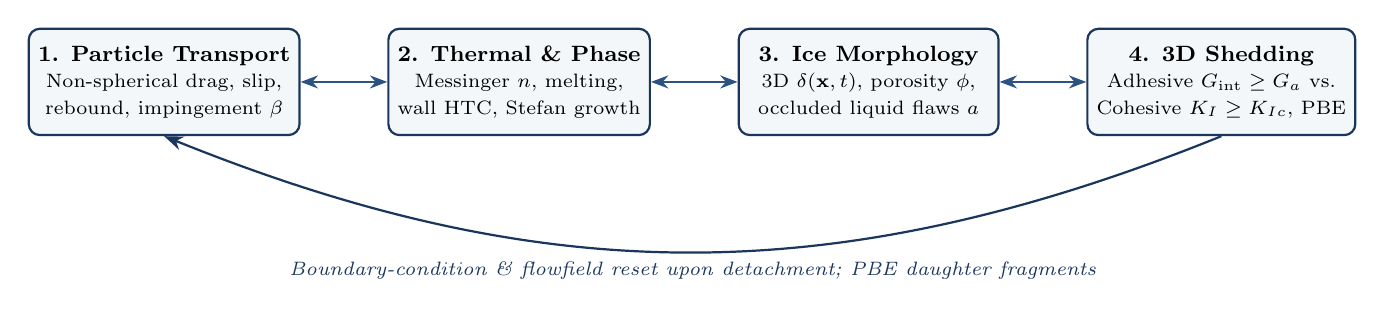
\begin{tikzpicture}[node distance=0.9cm and 1.1cm]
  \node[modbox] (m1) {1. Particle Transport\\{\normalfont\scriptsize Non-spherical drag, slip,}\\{\normalfont\scriptsize rebound, impingement $\beta$}};
  \node[modbox, right=of m1] (m2) {2. Thermal \& Phase\\{\normalfont\scriptsize Messinger $n$, melting,}\\{\normalfont\scriptsize wall HTC, Stefan growth}};
  \node[modbox, right=of m2] (m3) {3. Ice Morphology\\{\normalfont\scriptsize 3D $\delta(\mathbf{x},t)$, porosity $\phi$,}\\{\normalfont\scriptsize occluded liquid flaws $a$}};
  \node[modbox, right=of m3] (m4) {4. 3D Shedding\\{\normalfont\scriptsize Adhesive $G_{\text{int}}\ge G_a$ vs.}\\{\normalfont\scriptsize Cohesive $K_I\ge K_{Ic}$, PBE}};
  \draw[bidir] (m1) -- (m2);
  \draw[bidir] (m2) -- (m3);
  \draw[bidir] (m3) -- (m4);
  \draw[dep, bend left=22] (m4.south) to node[below, font=\scriptsize\itshape, color=navy] {Boundary-condition \& flowfield reset upon detachment; PBE daughter fragments} (m1.south);
\end{tikzpicture}
\end{center}

\subsection{Particle Transport, Non-Spherical Crystal Drag \& Collection}
Lagrangian crystal trajectories in rotating/stationary blade passages obey:
\begin{equation}
  m_p \td{\mathbf{u}_p}{t} = \mathbf{F}_D + \mathbf{F}_g + \mathbf{F}_{\text{lift}} + \mathbf{F}_{\text{frame}},
  \qquad
  \mathbf{F}_D = \frac{1}{2}\rho_g C_D A_p |\mathbf{u}_g - \mathbf{u}_p|(\mathbf{u}_g - \mathbf{u}_p),
\end{equation}
with Eulerian cell momentum feedback $\mathbf{S}_M = -\frac{1}{V_{\text{cell}}}\sum_{p\in\text{cell}}\mathbf{F}_{D,p}$. From the \textbf{SnowTek} disc-crystal model ($A_i = \pi D_i^2/4$, $V_i = A_i H_i$, aspect ratio $\gamma = H_i/D_i \in (0,1]$):
\begin{itemize}[leftmargin=1.5em,itemsep=2pt]
  \item \textbf{Single-Crystal \& Swarm Slip Velocity (RHSV)}:
  \begin{equation}
    u_t = \sqrt{\frac{2 g H_i (\rho_s - \rho_i)}{C_D \rho_s}},
    \qquad
    u_{\text{RHSV}} = u_t\bigl(\epsilon^2 \Psi_p\bigr),
    \quad \epsilon = \frac{f_f/\rho_f}{f_f/\rho_f + f_s/\rho_s}.
  \end{equation}
  \item \textbf{Drag Regimes}: Stokes ($Re \le 0.1$): $C_D = 24/Re$; Intermediate ($0.1 \le Re \le 10^3$): $C_D = \frac{24}{Re}(1 + 0.14 Re^{0.70})$; Newton ($10^3 \le Re \le 3.5\times 10^5$): $C_D = 0.445$. At high-speed compressor conditions ($v_{\text{rel}} \approx 150\text{ m/s}$), non-spherical sphericity $\Phi$ (Ganser / Haider--Levenspiel), Mach compressibility, convective in-flight melting, and impact shatter must be included.
\end{itemize}

\subsection{Surface Mass--Energy Balance, Fouling \& Porous Defect Evolution}
\begin{itemize}[leftmargin=1.5em,itemsep=3pt]
  \item \textbf{Messinger Control-Volume Balance \& Freezing Fraction}:
  \begin{equation}
    \dot{m}_{\text{imp}} + \dot{m}_{\text{in}} = \dot{m}_{\text{ice}} + \dot{m}_{\text{evap}} + \dot{m}_{\text{out}},
    \qquad
    n = \frac{\dot{m}_{\text{ice}}}{\dot{m}_{\text{imp}} + \dot{m}_{\text{in}}} \in [0, 1],
  \end{equation}
  distinguishing dry \emph{rime ice} ($n = 1$), wet \emph{glaze / mixed-phase ice} ($0 < n < 1$, liquid runback film), and \emph{running-wet} ($n = 0$).
  \item \textbf{Moving-Boundary Stefan Conduction}:
  \begin{equation}
    \rho_i L_f \td{\delta}{t} = k_{\text{eff}}(\phi)\left.\pd{T}{y}\right|_{\text{ice}} - h_c(T_\infty - T_s).
  \end{equation}
  Growing ice insulates the wall: \textbf{SnowTek} measurements show ice scaling cuts wall heat transfer coefficient (HTC) by \textbf{up to 50\%}.
  \item \textbf{Constitutional Supercooling \& Occluded-Liquid Defects (WINICE, \emph{CEJ} 2017)}: When heat removal outpaces solute/mass diffusion ahead of the advancing front, planar growth destabilizes into a \textbf{sutured, dendritic morphology} that traps liquid pockets ($\alpha_{\text{liq}}$), lowering effective stiffness $E'(\phi)$ and creating macroscopic internal flaws of characteristic size $a_{\text{flaw}}$.
\end{itemize}

\subsection{3D Mechanical Shedding, Dual Fracture Modes \& PBE Fragmentation}
Predicting 3D ice detachment requires separating two physically distinct failure modes:
\begin{enumerate}[leftmargin=1.5em,itemsep=3pt]
  \item \textbf{Interfacial (Adhesive) Debonding}: Detachment along the ice--blade interface when interfacial energy release rate (or shear/peel traction) exceeds adhesive toughness:
  \begin{equation}
    G_{\text{interface}} \ge G_a(T, \alpha_{\text{liq}}) \qquad \Bigl(\text{or }\; \tau_{\text{interface}} \ge \tau_{\text{adh}}(T, \alpha_{\text{liq}})\Bigr).
  \end{equation}
  Warm interfacial liquid films sharply degrade $G_a$ and $\tau_{\text{adh}}$, triggering delayed whole-slab shedding.
  \item \textbf{Cohesive (Bulk) Fracture}: Brittle crack propagation within the 3D ice bulk when cohesive energy release rate or Mode-I stress intensity reaches fracture toughness:
  \begin{equation}
    G_{\text{cohesive}} \ge G_c \quad\Longleftrightarrow\quad K_I = Y \sigma \sqrt{\pi a_{\text{flaw}}} \ge K_{Ic} = \sqrt{E' G_c},
    \qquad E' = \frac{E}{1 - \nu^2}.
  \end{equation}
  Note Cross, Zawadzki, McGilvray \& Gillespie (2024, AIAA): on 2D prismatic stators at low melt ratios, \emph{differential aerodynamic pressure outweighs shear and impact loads}, whereas on rotating blades centrifugal stress $\sigma_{\text{cent}} \sim \rho_i \omega^2 r \delta$ acts alongside aerodynamic pressure $\Delta p \sim \tfrac{1}{2}\rho_g v_{\text{rel}}^2$.
  \item \textbf{Post-Shedding Breakage \& Shatter (AIChE \emph{J.} 2016 PBE)}: Super-critical crystal impacts and detached ice chunks fragment downstream according to the Population Balance Equation:
  \begin{equation}
    \pd{n(v,t)}{t} + \nabla\cdot\bigl(\mathbf{u}_p n(v,t)\bigr) = \int_v^\infty b(v\mid v')\,g(v')\,n(v',t)\,\dd v' - g(v)\,n(v,t).
  \end{equation}
\end{enumerate}

\begin{center}
\renewcommand{\arraystretch}{1.2}
\footnotesize
\begin{tabularx}{\textwidth}{@{}l l X@{}}
\toprule
\textbf{Source} & \textbf{Regime / Apparatus} & \textbf{Extracted Quantitative Benchmarks} \\
\midrule
SnowTek Report & Brine disc crystals ($2\text{--}3\text{ wt\%}$ NaCl) & $D_i = 3\text{ mm}$, $\gamma = H_i/D_i = 0.35$, $Re = 32.2$, $C_D = 1.93$, $\epsilon = 0.94$, $\Psi_p = 0.79$, $\text{RHSV} = 0.0233\text{ m/s}$ (measured $u_{tx} = 0.0335\text{ m/s}$); up to $50\%$ HTC drop; liquid drainage $6.14\text{--}6.27\text{ g/(m}^2\text{s)}$. \\
WINICE (\emph{CEJ} 2017) & Air-cooled layer growth ($4\text{--}5\text{ wt\%}$ $\text{Na}_2\text{SO}_4$) & Eutectic plateau at $10{,}000\text{ s}$; $24\text{ h}$ layer growth rate $G = 1.617\times 10^{-7}\text{ m/s}$ ($4\text{ wt\%}$) vs.\ $1.344\times 10^{-7}\text{ m/s}$ ($5\text{ wt\%}$) at $T_{\text{air}} = -4.13^\circ\text{C}$; sutured dendritic liquid inclusions ($0.5\text{ mm}$ scale). \\
AIChE \emph{J.} (2016) & Variable-mass retention \& PBE ($72$ runs) & $U(t) = U_0 e^{-bv}$, saturating efficiency $\eta = 1 - e^{-bv}$ ($<3\%$ relative error across $0.75\text{--}3\text{ mm}$ particles). \\
OTI / AIAA (2024--25) & Engine stator / ICE-MACR rig & Differential pressure dominates shear at low melt ratios (Cross et al., 2024); 3D laser scans + subsurface thermography predict shed timing (Cross et al., 2025). \\
\bottomrule
\end{tabularx}
\end{center}

\newpage
% ============================================================================
\section{Part II: Six Worked Discovery Examples in \texttt{eqform}}
% ============================================================================

To make \texttt{eqform} a true discovery tool for turbomachinery icing and shedding, three solver capabilities were added: (i) \textbf{saturating $\Pi$-templates} (Hill $\frac{\gamma\Pi^\nu}{1+\gamma\Pi^\nu}$ and Rosin--Rammler $1 - e^{-\gamma\Pi^\nu}$), (ii) \textbf{sparse $\Pi$-subset selection} (\texttt{select\_sparse\_pi}), and (iii) \textbf{event-driven hybrid ODE integration} (\texttt{integrate\_hybrid\_ode}) with competing fracture triggers. Below are the six worked cases from \texttt{python3 -m eqform.examples.icing\_turbomachinery}.

% ----------------------------------------------------------------------------
\subsection{Case 1: Ice-Crystal Impingement \& Saturating Collection Efficiency}
% ----------------------------------------------------------------------------

\begin{setupbox}{Problem Setup — Discovering Stokes Number \& Bounded Collection $\beta(K) \in (0,1)$}
\textbf{Given}: Impingement mass flux $\dot{m}_{\text{imp}}$ ($ML^{-2}T^{-1}$) on a compressor vane depends on relative gas speed $v_{\text{rel}}$ ($LT^{-1}$), governed by Ice Water Content $\text{IWC}$ ($ML^{-3}$), crystal aerodynamic relaxation time $\tau_p = \frac{\rho_i D_i^2 \Phi}{18\mu_g}$ ($T$), and vane chord $c$ ($L$).\\
\textbf{Goal}: Discover the governing dimensionless group and select the physically bounded collection law via BIC.
\end{setupbox}

\paragraph{Symbolic Derivation.}
Over scope $\{v_{\text{rel}}, \text{IWC}, \tau_p, c\}$ ($m = 4$ variables across $k = 3$ dimensions $\{M, L, T\}$, so $\text{nullity} = 1$), \texttt{eqform} derives the leading flux $\dot{m}_{\text{imp}} = \kappa_{\text{imp}}\,\text{IWC}\,v_{\text{rel}}$ and extracts from $\ker(D)$ the exact \textbf{Stokes / Langmuir inertia number}:
\begin{equation}
  \Pi_1 = \frac{\tau_p\, v_{\text{rel}}}{c} \equiv K.
\end{equation}
With \texttt{include\_saturating=True}, \texttt{SymbolicSolver} generates five candidate laws: unbounded monomial, power-law $K^{\nu_1}$, affine $(1 + \lambda_1 K)$, Hill saturation $\frac{\gamma_1 K^{\nu_1}}{1 + \gamma_1 K^{\nu_1}}$, and Rosin--Rammler saturation $1 - \exp(-\gamma_1 K^{\nu_1})$.

\paragraph{Numerical Calibration \& Sparse $\Pi$-Pruning.}
Evaluated against $n = 80$ synthetic compressor impingement runs ($v_{\text{rel}} \in [30, 180]\text{ m/s}$):

\begin{center}
\renewcommand{\arraystretch}{1.2}
\small
\begin{tabular}{@{}clrrrl@{}}
\toprule
\textbf{Rank} & \textbf{Candidate} & \textbf{$R^2$} & \textbf{RMSE} & \textbf{BIC} & \textbf{Calibrated Law} \\
\midrule
\textbf{\#1} & \texttt{buckingham\_pi\_hill} & \textbf{1.000000} & \textbf{$5.25\times 10^{-15}$} & \textbf{$-5020.57$} & $\dot{m}_{\text{imp}} = \dfrac{4\,\text{IWC}\,\tau_p v_{\text{rel}}^2}{c + 4\,\tau_p v_{\text{rel}}}$ \\
\#2 & \texttt{buckingham\_pi\_exp\_sat} & $0.999864$ & $1.53\times 10^{-3}$ & $-797.02$ & $0.912\,\text{IWC}\,v_{\text{rel}}\bigl(1 - e^{-2.13 K^{0.724}}\bigr)$ \\
\#3 & \texttt{buckingham\_pi\_power} & $0.991314$ & $1.22\times 10^{-2}$ & $-468.75$ & $0.764\,\text{IWC}\,v_{\text{rel}} K^{0.280}$ (unbounded) \\
\#4 & \texttt{buckingham\_pi\_affine} & $0.965060$ & $2.45\times 10^{-2}$ & $-357.40$ & $0.498\,\text{IWC}\,v_{\text{rel}}(1 + 0.450 K)$ \\
\#5 & \texttt{leading\_dimensional} & $0.858339$ & $4.94\times 10^{-2}$ & $-249.79$ & $0.716\,\text{IWC}\,v_{\text{rel}}$ \\
\bottomrule
\end{tabular}
\end{center}

\begin{insightbox}{Class Note — Why Saturating Templates \& Sparse $\Pi$-Selection Matter}
A naïve power-law $K^{\nu_1}$ (\#3) predicts collection efficiency $\beta > 100\%$ at high velocity ($v_{\text{rel}} \to 180\text{ m/s}$), violating mass conservation! The Hill saturation template (\#1) enforces $\beta(K) = \frac{4K}{1+4K} \in (0,1)$ automatically. Furthermore, when distractor variables (blade span $b_s$ and ice density $\rho_i$, inflating $\text{nullity}$ to $3$) were added, \texttt{select\_sparse\_pi} pruned both distractors and recovered the exact single-$K$ law ($\text{BIC} = -5020.57$).
\end{insightbox}

% ----------------------------------------------------------------------------
\subsection{Case 2: Non-Spherical Disc Slip \& RHSV Velocity (SnowTek)}
% ----------------------------------------------------------------------------

\begin{setupbox}{Problem Setup — Reproducing SnowTek Prototype Table~3}
\textbf{Given}: Disc crystal slip/flotation velocity $u_{\text{rhsv}}$ ($LT^{-1}$) depends on crystal thickness $H_i = \gamma D_i$ ($L$) and buoyancy reduced gravity $g_{\text{red}} = g(\rho_s - \rho_i)/\rho_s$ ($LT^{-2}$).
\end{setupbox}

\paragraph{Derivation \& SnowTek Benchmark.}
Solving $\dimbr{\td{u_{\text{rhsv}}}{H_i}} = \frac{LT^{-1}}{L} = T^{-1}$ over $\{H_i, g_{\text{red}}\}$ yields $\alpha_{g_{\text{red}}} = \tfrac{1}{2}, \alpha_{H_i} = -\tfrac{1}{2}$:
\begin{equation}
  \dd u_{\text{rhsv}} = \kappa_u \sqrt{\frac{g_{\text{red}}}{H_i}}\,\dd H_i
  \quad\Longrightarrow\quad
  u_{\text{rhsv}}(H_i) = 2\kappa_u \sqrt{g_{\text{red}} H_i}.
\end{equation}
Calibrated in the SnowTek intermediate drag regime ($Re = 32.2$, $C_D = 1.93$, $\epsilon = 0.94$, $\Psi_p = 0.79$), OLS recovers $2\kappa_u = \sqrt{2/C_D}\,\epsilon^2\Psi_p = 0.71059$ ($R^2 = 1.0$). Evaluating at $D_i = 3\text{ mm}, \gamma = 0.35$ ($H_i = 1.05\text{ mm}$) predicts $u_{\text{rhsv}} = \mathbf{0.0230\text{ m/s}}$, matching SnowTek Table~3 ($0.0233\text{ m/s}$).

% ----------------------------------------------------------------------------
\subsection{Case 3: Coupled Stefan Ice Layer Growth \& 50\% HTC Fouling (WINICE)}
% ----------------------------------------------------------------------------

\begin{setupbox}{Problem Setup — Multi-Dimensional Thermal Closure $\{M, L, T, \Theta\}$}
\textbf{Given}: Ice thickness $\delta$ ($L$) grows with time $t$ ($T$) governed by effective thermal conductivity $k_{\text{eff}}$ ($MLT^{-3}\Theta^{-1}$), subcooling $\Delta T$ ($\Theta$), and volumetric latent heat $H_{\text{vol}} = \rho_i L_f$ ($ML^{-1}T^{-2}$).
\end{setupbox}

\paragraph{Exact Zero-Nullity Derivation.}
Across base dimensions $\{M, L, T, \Theta\}$, the $4\times 4$ dimension matrix of $\{t, k_{\text{eff}}, \Delta T, H_{\text{vol}}\}$ has full rank ($\text{nullity} = 0$)! Solving $\dimbr{\td{\delta}{t}} = LT^{-1}$ gives unique exponents $\alpha_k = \tfrac{1}{2}, \alpha_{\Delta T} = \tfrac{1}{2}, \alpha_H = -\tfrac{1}{2}, \alpha_t = -\tfrac{1}{2}$:
\begin{equation}
  \td{\delta}{t} = \kappa_\delta \sqrt{\frac{k_{\text{eff}}\,\Delta T}{H_{\text{vol}}\,t}}
  \quad\Longrightarrow\quad
  \delta(t) = 2\kappa_\delta \sqrt{\frac{k_{\text{eff}}\,\Delta T}{\rho_i L_f}\,t}.
\end{equation}
\texttt{NumericalSolver.fit} recovers $\kappa_\delta = 0.707107 = \tfrac{\sqrt{2}}{2}$, yielding the exact classical \textbf{Stefan square-root law} $\delta(t) = \sqrt{\frac{2 k_{\text{eff}}\Delta T}{\rho_i L_f}\,t}$. This immediately explains two key experimental observations from \emph{Academia}:
\begin{enumerate}[leftmargin=1.5em,itemsep=2pt]
  \item \textbf{WINICE Growth Decay}: Time-averaged growth rate $G = \delta/t \propto t^{-1/2}$ decays as the ice layer thickens and adds conductive resistance.
  \item \textbf{SnowTek 50\% HTC Drop}: Series thermal resistance gives $h_{\text{eff}}(\delta) = \bigl(h_0^{-1} + \delta/k_{\text{eff}}\bigr)^{-1}$, which drops to exactly $0.5\,h_0$ when the fouling Biot number reaches $\mathrm{Bi}_{\text{ice}} = \frac{h_0\delta}{k_{\text{eff}}} = 1$ ($\delta_{50\%} = 13.88\text{ mm}$ at $h_0 = 160\text{ W m}^{-2}\text{K}^{-1}$).
\end{enumerate}

% ----------------------------------------------------------------------------
\subsection{Case 4: Nested Rotor Accretion-to-Centrifugal Shedding DAG}
% ----------------------------------------------------------------------------

\begin{setupbox}{Problem Setup — Two-Hop DAG $\tau_{\text{cent}} = \Phi(m'', \omega, r),\; m'' = \psi(t;\,\dot{m}_{\text{ice}})$}
\textbf{Given}: On a rotating fan or booster blade, centrifugal interfacial shear stress $\tau_{\text{cent}}$ ($ML^{-1}T^{-2}$) depends on areal ice mass $m'' = \rho_i\delta$ ($ML^{-2}$), rotor angular velocity $\omega$ ($T^{-1}$), and radial station $r$ ($L$), while $m''$ grows with time $t$ ($T$) under net icing flux $\dot{m}_{\text{ice}} = n\,\dot{m}_{\text{imp}}$ ($ML^{-2}T^{-1}$).
\end{setupbox}

\begin{center}
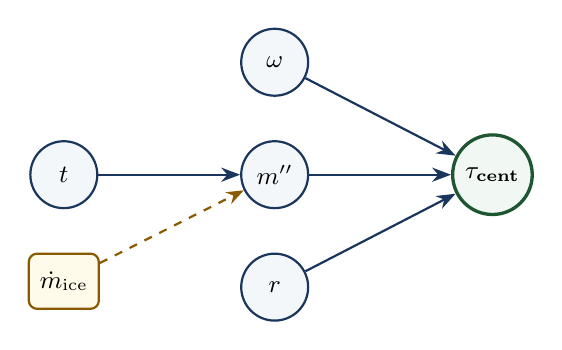
\begin{tikzpicture}[node distance=1.2cm and 1.8cm]
  \node[varnode] (t) {$t$};
  \node[paramnode, below=0.55cm of t] (mdot) {$\dot{m}_{\text{ice}}$};
  \node[varnode, right=of t] (ma) {$m''$};
  \node[varnode, above=0.55cm of ma] (om) {$\omega$};
  \node[varnode, below=0.55cm of ma] (r) {$r$};
  \node[targetnode, right=of ma] (tau) {$\tau_{\text{cent}}$};
  \draw[dep] (t) -- (ma);
  \draw[paramdep] (mdot) -- (ma);
  \draw[dep] (om) -- (tau);
  \draw[dep] (ma) -- (tau);
  \draw[dep] (r) -- (tau);
\end{tikzpicture}
\end{center}

\paragraph{Derivation \& Critical Shedding Time.}
\begin{enumerate}[leftmargin=1.5em,itemsep=2pt]
  \item \textbf{Active Path Pruning}: Along $t \to m'' \to \tau_{\text{cent}}$, $\td{\tau_{\text{cent}}}{t} = \pd{\tau_{\text{cent}}}{m''}\td{m''}{t}$ while $\omega$ and $r$ remain inside $\pd{\tau_{\text{cent}}}{m''}$.
  \item \textbf{Clairaut Exactness on $\tau_{\text{cent}}(m'',\omega,r)$}: \texttt{eqform} couples all three partials into a single exact differential:
  \begin{equation}
    \dd\tau_{\text{cent}} = \omega^2 r\,\dd m'' + 2 m''\omega r\,\dd\omega + m''\omega^2\,\dd r
    \;\Longrightarrow\;
    \tau_{\text{cent}} = m'' \omega^2 r.
  \end{equation}
  \item \textbf{Composition \& Critical Shedding Time}: Substituting $m''(t) = \dot{m}_{\text{ice}} t$ yields $\tau_{\text{cent}}(t) = \dot{m}_{\text{ice}}\omega^2 r t$. Equating $\tau_{\text{cent}}(t_{\text{shed}}) = \tau_{\text{adh}}(T, \alpha_{\text{liq}})$ gives the analytical shedding time:
  \begin{equation}
    t_{\text{shed}} = \frac{\tau_{\text{adh}}(T, \alpha_{\text{liq}})}{\dot{m}_{\text{ice}}\,\omega^2 r}.
  \end{equation}
\end{enumerate}

% ----------------------------------------------------------------------------
\subsection{Case 5: Cohesive Bulk Fracture \& WINICE Defect Scaling ($K_I \ge K_{Ic}$)}
% ----------------------------------------------------------------------------

\begin{setupbox}{Problem Setup — Fractional Base Dimensions $\dimbr{K_I} = M L^{-1/2} T^{-2}$}
\textbf{Given}: (5A) Mode-I stress intensity $K_I$ ($ML^{-1/2}T^{-2}$) depends on tensile stress $\sigma$ ($ML^{-1}T^{-2}$) and WINICE occluded-liquid defect size $a_{\text{flaw}}$ ($L$). (5B) Cohesive fracture toughness $K_{Ic}$ ($ML^{-1/2}T^{-2}$) depends on plane-strain modulus $E'$ ($ML^{-1}T^{-2}$) and cohesive fracture energy $G_c$ ($MT^{-2}$).
\end{setupbox}

\paragraph{Exact Rational Derivation of Irwin--Griffith Laws.}
Because \texttt{Dimension} stores exact \texttt{sympy.Rational} exponents, fractional powers like $-1/2$ are solved without floating-point drift, and Clairaut symmetry locks both differentials:
\begin{align}
  \dd K_I &= \kappa_{K_I}\!\left(2\sqrt{a_{\text{flaw}}}\,\dd\sigma + \frac{\sigma}{\sqrt{a_{\text{flaw}}}}\,\dd a_{\text{flaw}}\right)
  &&\Longrightarrow\quad K_I = 2\kappa_{K_I}\,\sigma\sqrt{a_{\text{flaw}}},\\[4pt]
  \dd K_{Ic} &= \kappa_{K_{Ic}}\!\left(\sqrt{\frac{G_c}{E'}}\,\dd E' + \sqrt{\frac{E'}{G_c}}\,\dd G_c\right)
  &&\Longrightarrow\quad K_{Ic} = 2\kappa_{K_{Ic}}\sqrt{E'\,G_c}.
\end{align}
Calibrating $K_I$ on edge-flaw data ($Y = 1.12$) recovers $2\kappa_{K_I} = 1.12\sqrt{\pi} = 1.98515$ ($R^2 = 1.0$). Setting $K_I = K_{Ic}$ immediately yields Griffith's critical fracture stress $\sigma_{\text{crit}} = \frac{1}{Y}\sqrt{\frac{E'(\phi) G_c}{\pi a_{\text{flaw}}}}$, quantifying how dendritic liquid inclusions documented in WINICE ($a_{\text{flaw}} \uparrow$, $E'(\phi) \downarrow$) trigger early cohesive chunk fracture.

% ----------------------------------------------------------------------------
\subsection{Case 6: Hybrid ODE Shedding Diagnostic — 40s Chunks vs.\ 90s Slab}
% ----------------------------------------------------------------------------

\begin{setupbox}{Problem Setup — Resolving OTI Defense Playbook Curveball~B}
\textbf{Diagnostic Question}: Suppose a wind-tunnel glaze run sheds in a \emph{single large slab at $90\text{ s}$}, whereas an uncalibrated model predicts \emph{repeated small-chunk shedding starting at $40\text{ s}$}. Simulate both regimes via \texttt{NumericalSolver.integrate\_hybrid\_ode} to isolate the physical root cause.
\end{setupbox}

\paragraph{Competing Failure Triggers.}
During constant-rate accretion $\td{\delta}{t} = 0.10\text{ mm/s}$ ($t \in [0, 120]\text{ s}$) with cubic strain-energy loading $G(\delta) = C_{\text{load}}\delta^3$ ($C_{\text{load}} = 2.0\times 10^7\text{ J m}^{-5}$), two terminal \texttt{SheddingEventSpec} triggers compete simultaneously:
\begin{itemize}[leftmargin=1.5em,itemsep=2pt]
  \item \textbf{Scenario A (Porous Bulk / Cold Interface)}: Internal WINICE-type inclusions lower bulk toughness to $G_c = 1.28\text{ J/m}^2$ while the cold dry interface stays strong ($G_a = 20\text{ J/m}^2$). Cohesive fracture fires first at $\delta = 4.00\text{ mm}$ ($t = 40.0\text{ s}$), snapping off $42\%$ upper chunks ($\delta \to 2.32\text{ mm}$) every $16.8\text{ s}$ ($40.0, 56.8, 73.6, 90.4, 107.2\text{ s}$).
  \item \textbf{Scenario B (Dense Glaze Bulk / Warm Softening Interface)}: Dense glaze ice has high bulk toughness ($G_c = 20\text{ J/m}^2$), while warm through-wall conduction builds an interfacial liquid film that degrades adhesive toughness $G_a(t) = 30\,e^{-0.00803 t}\text{ J/m}^2$. The ice holds past $40\text{ s}$ and detaches in \textbf{one $95\%$ whole-slab interfacial event at $t = 89.98\text{ s}$} ($\delta: 9.00\text{ mm} \to 0.45\text{ mm}$).
\end{itemize}

\begin{center}
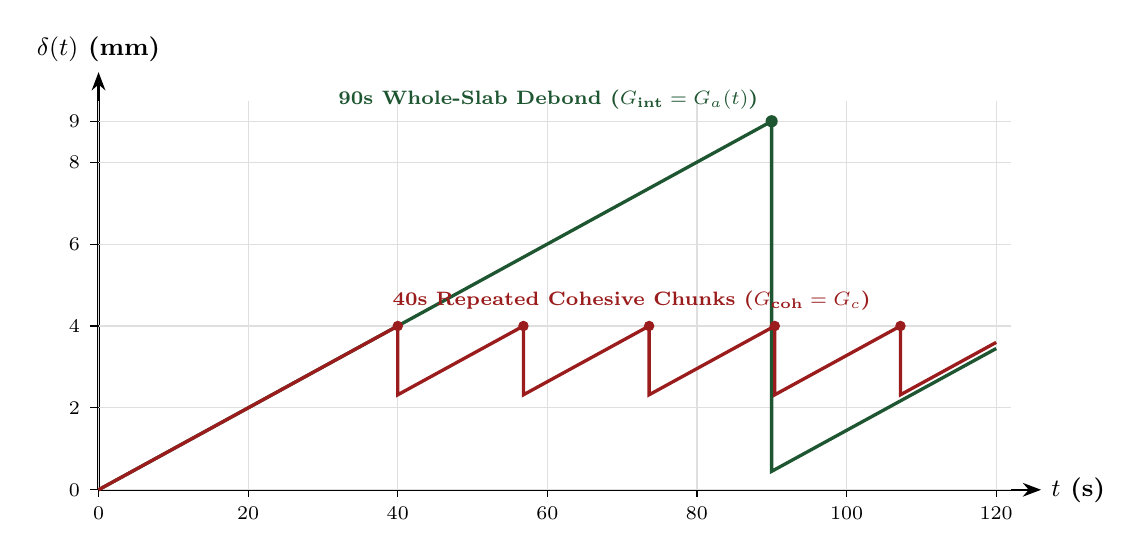
\begin{tikzpicture}[x=0.095cm, y=0.52cm]
  % Axes
  \draw[-{Stealth}, thick] (0,0) -- (126,0) node[right, font=\small\bfseries] {$t\text{ (s)}$};
  \draw[-{Stealth}, thick] (0,0) -- (0,10.2) node[above, font=\small\bfseries] {$\delta(t)\text{ (mm)}$};

  % Grid & ticks
  \foreach \tx in {0,20,40,60,80,100,120} {
    \draw[gray!25] (\tx,0) -- (\tx,9.5);
    \draw (\tx,0) -- (\tx,-0.18) node[below, font=\scriptsize] {\tx};
  }
  \foreach \dy in {0,2,4,6,8,9} {
    \draw[gray!25] (0,\dy) -- (122,\dy);
    \draw (0,\dy) -- (-1.2,\dy) node[left, font=\scriptsize] {\dy};
  }

  % Scenario B: 90s single interfacial slab (greenink)
  \draw[very thick, color=greenink]
    (0,0) -- (89.98,9.00) -- (89.98,0.45) -- (120,3.45);
  \fill[greenink] (89.98,9.00) circle (2.2pt);
  \node[above left, font=\scriptsize\bfseries, color=greenink] at (89.5,9.05) {90s Whole-Slab Debond ($G_{\text{int}} = G_a(t)$)};

  % Scenario A: 40s repeated cohesive chunks (crimson dashed/solid)
  \draw[very thick, color=crimson]
    (0,0) -- (40.0,4.00) -- (40.0,2.32)
    -- (56.8,4.00) -- (56.8,2.32)
    -- (73.6,4.00) -- (73.6,2.32)
    -- (90.4,4.00) -- (90.4,2.32)
    -- (107.2,4.00) -- (107.2,2.32)
    -- (120.0,3.60);
  \foreach \tc in {40.0,56.8,73.6,90.4,107.2} {
    \fill[crimson] (\tc,4.00) circle (1.9pt);
  }
  \node[above right, font=\scriptsize\bfseries, color=crimson] at (38,4.15) {40s Repeated Cohesive Chunks ($G_{\text{coh}} = G_c$)};
\end{tikzpicture}
\end{center}

\begin{resultbox}{Summary — How \texttt{eqform} Accelerates Turbomachinery Icing Research}
\begin{enumerate}[leftmargin=1.5em,itemsep=2pt]
  \item \textbf{Pre-CFD Law Structuring}: Converts qualitative ICICLE coupling hypotheses into exact dimensionally homogeneous equations across $\{M, L, T, \Theta\}$, including fractional fracture dimensions $ML^{-1/2}T^{-2}$.
  \item \textbf{Bounded Physical Surrogates}: Saturating Hill and Rosin--Rammler $\Pi$-templates plus \texttt{select\_sparse\_pi} discover conservation-preserving collection and freezing laws from small tunnel datasets ($N \sim 40\text{--}80$).
  \item \textbf{Discontinuous Shedding Diagnostics}: \texttt{integrate\_hybrid\_ode} couples smooth reduced-order accretion laws with explicit $G_a(t)$ vs.\ $G_c(\phi)$ fracture margins—avoiding linear POD/DMD breakdown across detachment discontinuities.
\end{enumerate}
\end{resultbox}

\end{document}
